% ==========================================================================
%  MaayaTrain — IEEEtran Conference Paper
%  Title B: Async-DiLoCo with Network-Adaptive Sharding and Block-Wise
%           Gradient Quantization for Edge-Distributed LLM Training
% ==========================================================================
\documentclass[10pt,conference]{IEEEtran}

% --- Packages ---
\usepackage{amsmath,amssymb,amsfonts}
\usepackage{graphicx}
\usepackage{algorithmic}
\usepackage{algorithm}
\usepackage{booktabs}
\usepackage{url}
\usepackage{hyperref}
\usepackage{xcolor}
\usepackage{multirow}
\usepackage{balance}

% Compact lists inside algorithms
\renewcommand{\algorithmiccomment}[1]{\hfill\textit{// #1}}

\begin{document}

% ===== TITLE =====
\title{Async-DiLoCo with Network-Adaptive Sharding and Block-Wise\\
Gradient Quantization for Edge-Distributed LLM Training}

% ===== AUTHORS =====
\author{
  \IEEEauthorblockN{Akhil Ageer}
  \IEEEauthorblockA{
    Department of Computer Science\\
    Kean University\\
    Union, New Jersey, USA\\
    ai@computer.org
  }
}

\maketitle

% ====================================================================
%  ABSTRACT
% ====================================================================
\begin{abstract}
Training large language models (LLMs) conventionally requires tightly coupled
GPU clusters interconnected via InfiniBand, imposing prohibitive capital costs
that preclude participation by independent researchers and academic
institutions. We present \textbf{MaayaTrain}, an open-source distributed
training framework that enables collaborative training of GPT-scale language
models across heterogeneous consumer hardware---spanning CUDA, Apple~MPS,
Intel~XPU, AMD~ROCm, and CPU backends---connected over commodity Wi-Fi
networks. Building upon the DiLoCo algorithm, MaayaTrain introduces four
novel systems-level contributions:
\textbf{(i)}~\emph{Compute-Proportional Async-DiLoCo}, which replaces
fixed-step synchronization with a time-bounded window where each worker's
pseudo-gradient is weighted by its local step count, achieving $>$95\%
compute utilization on heterogeneous clusters versus $\sim$20\% for
synchronous baselines;
\textbf{(ii)}~\emph{Network-Aware Dynamic Sharding}, which monitors
real-time TCP round-trip times via heartbeat probes and adapts the streaming
shard count from 1 to~16 using a piecewise doubling/halving policy;
\textbf{(iii)}~\emph{Outlier-Resilient Block-Wise INT8 Quantization}, which
partitions pseudo-gradient tensors into 128-element blocks with independent
per-block scaling, surviving the heavy-tailed outlier distributions
characteristic of AdamW training and achieving 8--12$\times$ compression
with zstandard entropy coding; and
\textbf{(iv)}~\emph{Stream-Chunked Median Aggregation}, which computes
coordinate-wise median for Byzantine fault tolerance in fixed-size chunks,
reducing peak memory from $O(n \times P)$ to $O(n \times C)$ and preventing
CPU out-of-memory failures on consumer devices.
The framework supports GPT-2 class models (124M--774M parameters) and is
validated through a comprehensive test suite across all subsystems.
\end{abstract}

\begin{IEEEkeywords}
Distributed Training, Large Language Models, DiLoCo, Asynchronous
Optimization, Gradient Quantization, Network-Adaptive Systems, Byzantine
Fault Tolerance, Consumer Hardware
\end{IEEEkeywords}

% ====================================================================
%  I. INTRODUCTION
% ====================================================================
\section{Introduction}
\label{sec:introduction}

\subsection{Motivation}

The training of modern large language models represents one of the most
compute-intensive workloads in contemporary machine learning. Training a
frontier model such as GPT-4 or LLaMA-3 requires thousands of high-end
NVIDIA~H100 GPUs operating in concert for weeks to months, with total costs
reaching tens of millions of dollars~\cite{touvron2023llama}. The fundamental
assumption of traditional distributed training---that all devices are
co-located in a single datacenter with high-bandwidth interconnects
(100+~Gb/s InfiniBand or NVLink)---imposes prohibitive capital and operational
costs, constraining participation to well-funded organizations.

Simultaneously, the aggregate computational capacity of the world's consumer
devices---laptops, workstations, gaming PCs, and Apple Silicon
Macs---substantially exceeds that available in centralized datacenters. An
NVIDIA~RTX~4090 delivers approximately 82.6~TFLOPS~(FP32), and Apple's M4~Pro
delivers approximately 8.7~TFLOPS, yet this aggregate capacity remains
underutilized for collaborative model training.

The bottleneck is not compute but \emph{communication}. Standard data-parallel
training~(DDP) synchronizes gradients at every step, requiring sustained
bandwidth of approximately 50~GB/s for a 124M~parameter
model~\cite{rajbhandari2020zero}. Consumer networks (Wi-Fi~6, home Ethernet)
provide only 0.1--1.0~GB/s---a gap of 50--500$\times$.

\subsection{Contributions}

We present MaayaTrain, a framework that bridges this gap through the following
contributions:

\begin{enumerate}
  \item \textbf{Compute-Proportional Async-DiLoCo.} We replace the
    synchronous fixed-step inner loop of DiLoCo with a time-bounded window.
    Each worker trains for a fixed wall-clock duration, and the coordinator
    aggregates pseudo-gradients weighted by local step count. This solves
    Amdahl's Law on heterogeneous clusters, achieving $>$95\% utilization
    where synchronous baselines achieve $\sim$20\% with 10$\times$ speed
    disparity (Section~\ref{sec:compute-proportional}).

  \item \textbf{Network-Aware Dynamic Sharding.} We extend Streaming
    DiLoCo~\cite{douillard2025streaming} with runtime shard adaptation based
    on cluster-wide TCP round-trip time monitoring. The shard count adapts
    from 1 to~16 using a piecewise policy, reducing per-message payload to
    $\sim$3.9~MB under congestion (Section~\ref{sec:dynamic-sharding}).

  \item \textbf{Outlier-Resilient Block-Wise INT8 Quantization.} Adapting the
    block-wise quantization paradigm from weight compression
    (QLoRA~\cite{dettmers2023qlora}) to gradient compression, we partition
    pseudo-gradient tensors into 128-element blocks with independent
    min--max affine scaling. Combined with zstandard entropy coding, this
    achieves 8--12$\times$ total compression while confining outlier damage
    to individual blocks (Section~\ref{sec:blockwise-int8}).

  \item \textbf{Stream-Chunked Median Aggregation.} We implement a
    memory-safe coordinate-wise median that processes worker tensors in
    fixed-size chunks of $5{\times}10^6$ elements, reducing peak memory by
    155$\times$ compared to na\"ive stacking
    (Section~\ref{sec:chunked-median}).
\end{enumerate}

\subsection{Paper Organization}

Section~\ref{sec:related} surveys related work.
Section~\ref{sec:framework} formalizes the algorithmic framework with full
mathematical definitions of all four contributions.
Section~\ref{sec:architecture} details the system architecture.
Section~\ref{sec:evaluation} presents the evaluation methodology.
Section~\ref{sec:conclusion} concludes.


% ====================================================================
%  II. RELATED WORK
% ====================================================================
\section{Related Work}
\label{sec:related}

\subsection{Synchronous Distributed Training}

Traditional distributed training employs data parallelism with synchronous
gradient aggregation via AllReduce~\cite{li2020pytorch}. PyTorch's
DistributedDataParallel~(DDP) and Fully Sharded Data Parallelism~(FSDP) are
industry standards, achieving near-linear scaling on co-located clusters with
NVLink/InfiniBand. However, these methods require gradient synchronization at
every training step, with bandwidth proportional to model size:
\begin{equation}
  \text{BW}_{\text{DDP}} = \frac{2 \cdot P \cdot 4\;\text{bytes}}{t_{\text{step}}}
  \approx 50\;\text{GB/s for}\;P{=}124\text{M}
\end{equation}
This renders DDP infeasible over consumer networks.

\subsection{DiLoCo: Distributed Low-Communication Training}

Douillard et al.~\cite{douillard2023diloco} introduced DiLoCo, decoupling
local training from global synchronization. Workers train independently for
$H$ steps (typically 500) before synchronizing, reducing communication by a
factor of $H$. DiLoCo employs a bi-level optimization: an inner AdamW
optimizer~\cite{loshchilov2019adamw} for local training, and an outer
Nesterov~SGD~\cite{nesterov1983} for global aggregation of pseudo-gradients
$\Delta\theta = \theta_{\text{global}} - \theta_{\text{local}}$. The original
work demonstrated convergence parity with DDP on language modeling tasks up to
400M parameters. Jaghouar et al.~\cite{jaghouar2024opendiloco} validated
DiLoCo at scale in OpenDiLoCo, training across two continents with
90--95\% compute utilization.

\subsection{Streaming DiLoCo}

Douillard et al.~\cite{douillard2025streaming} extended DiLoCo with streaming
synchronization, splitting parameters into $K$ shards for incremental sync,
reducing peak bandwidth by $K\!\times$. They further demonstrated that 4-bit
outer gradient quantization is viable at scale.

\subsection{Asynchronous and Federated Aggregation}

The broader field of Federated Learning~(FL), pioneered by McMahan et
al.~\cite{mcmahan2017fedavg} with FedAvg, shares DiLoCo's bi-level
optimization structure. Recent work on asynchronous FL has introduced
\emph{buffered} aggregation~\cite{nguyen2022fedbuff}, where the server
aggregates updates as they arrive without waiting for all clients. CASA
\cite{casa2024kdd} extends this with dynamic clustering under asynchrony at
KDD~2024. Our compute-proportional weighting (Section
\ref{sec:compute-proportional}) is architecturally related to buffered
asynchronous aggregation but employs an explicit step-count weighting scheme
rather than staleness-based decay.

\subsection{Gradient Compression}

Gradient compression has been extensively studied: Top-$K$ sparsification
\cite{aji2017sparse}, QSGD~\cite{alistarh2017qsgd}, and 1-bit
SGD~\cite{seide2014onebit} reduce communication at the cost of gradient
quality. GaLore~\cite{zhao2024galore} takes a fundamentally different
approach, projecting gradients into a low-rank subspace to reduce optimizer
state memory by 65.5\%. We distinguish our work from GaLore along the
\emph{memory-vs.-communication} axis: GaLore targets local optimizer memory,
while our block-wise INT8 targets wire-level bandwidth reduction. The two
approaches are complementary.

Block-wise quantization for neural network weights was formalized by Dettmers
et al.~\cite{dettmers2023qlora} in QLoRA, which introduced NF4 with
64-element blocks. Our work adapts the block-wise paradigm from weight
compression to \emph{gradient} compression, using 128-element blocks with
min--max affine INT8 scaling rather than NF4's absmax-centered scheme. This
design choice reflects the different statistical properties of gradients
(heavier tails, non-normal distributions) compared to weights.

\subsection{Byzantine Fault Tolerance}

Blanchard et al.~\cite{blanchard2017byzantine} formalized Byzantine-resilient
gradient descent with Krum. Yin et al.~\cite{yin2018byzantine} proposed
coordinate-wise median as a computationally efficient alternative with
provable robustness: the aggregated gradient remains close to the true
gradient even when up to $\lfloor(n{-}1)/3\rfloor$ workers submit arbitrary
updates. MaayaTrain implements coordinate-wise median with a stream-chunked
variant that avoids out-of-memory failures on consumer hardware.


% ====================================================================
%  III. ALGORITHMIC FRAMEWORK
% ====================================================================
\section{Algorithmic Framework}
\label{sec:framework}

\subsection{Problem Formulation}

We consider the standard autoregressive language modeling objective. Given a
corpus $\mathcal{D} = \{x_1, x_2, \ldots, x_N\}$ of text sequences, we
minimize:
\begin{equation}
  \mathcal{L}(\theta) = -\frac{1}{N}\sum_{i=1}^{N}\sum_{t=1}^{T}
  \log p_\theta(x_{i,t} \mid x_{i,<t})
  \label{eq:lm-loss}
\end{equation}
where $\theta$ denotes model parameters, $T$ is the sequence length, and
$p_\theta$ is the autoregressive probability.

In the distributed setting with $n$ workers, each worker $k$ has access to a
local data shard $\mathcal{D}_k$. Workers train independently and synchronize
periodically via the DiLoCo protocol~\cite{douillard2023diloco}.

\subsection{Base DiLoCo Protocol}

MaayaTrain implements DiLoCo as a bi-level optimization. The inner optimizer
uses AdamW~\cite{loshchilov2019adamw} with decoupled weight decay. The inner
optimizer state is \emph{reset} at the start of each round, preventing stale
momentum from corrupting gradient estimates---a design validated by both
DiLoCo~\cite{douillard2023diloco} and OpenDiLoCo~\cite{jaghouar2024opendiloco}.

The outer step uses Nesterov momentum~\cite{nesterov1983} with momentum
coefficient $\beta = 0.9$ and learning rate $\eta = 0.7$:
\begin{align}
  v_t &= \beta \cdot v_{t-1} + \Delta\theta_{\text{agg}} \label{eq:momentum}\\
  \theta_{\text{global}} &\leftarrow \theta_{\text{global}}
    - \eta \cdot (\Delta\theta_{\text{agg}} + \beta \cdot v_t)
  \label{eq:nesterov}
\end{align}
where $\Delta\theta_{\text{agg}}$ is the aggregated pseudo-gradient.

% --- CONTRIBUTION 1 ---
\subsection{Compute-Proportional Async-DiLoCo}
\label{sec:compute-proportional}

In standard DiLoCo, all workers execute exactly $H$ inner steps before
synchronization. On heterogeneous clusters, this creates an Amdahl's Law
bottleneck: the slowest worker dictates round duration, and faster workers
idle while waiting. With a 10$\times$ speed disparity (e.g., RTX~4090 vs.
Apple~M4), synchronous utilization degrades to approximately 20\%.

\textbf{Time-Bounded Window.} We replace the fixed step count $H$ with a
fixed wall-clock window $T_{\text{window}}$ (default 60\,s). Each worker $k$
executes as many inner steps $h_k$ as its hardware permits within
$T_{\text{window}}$.

\textbf{Step-Count Weighting.} The coordinator aggregates pseudo-gradients
with weights proportional to each worker's compute contribution:
\begin{equation}
  w_k = \frac{h_k}{\displaystyle\sum_{j=1}^{n} h_j},
  \quad k = 1, \ldots, n
  \label{eq:weights}
\end{equation}
\begin{equation}
  \Delta\theta_{\text{agg}} = \sum_{k=1}^{n} w_k \cdot \Delta\theta_k
  \label{eq:weighted-agg}
\end{equation}

\textbf{Utilization Guarantee.} Let $\mathcal{C}_k$ be the theoretical peak
throughput (steps/sec) of worker $k$. The cluster compute utilization over
the window $T_{\text{window}}$ is:
\begin{equation}
  U_{\text{async}} = \frac{\sum_{k=1}^{n} h_k}
  {T_{\text{window}} \sum_{k=1}^{n} \mathcal{C}_k} \approx 1.0
  \label{eq:utilization}
\end{equation}
versus the synchronous baseline
$U_{\text{sync}} = \frac{n \cdot h_{\min}}
{T_{\text{window}} \sum_{k=1}^{n} \mathcal{C}_k}$,
which degrades severely when
$\max(\mathcal{C}_k) \gg \min(\mathcal{C}_k)$.

\textbf{FP32 Accumulation.} All weighted aggregation is performed in FP32
(IEEE~754 binary32) to prevent overflow when accumulating many workers'
gradients. FP16 saturates at $\max_{\text{fp16}} = 65{,}504$; summing $n$
worker pseudo-gradients can easily exceed this bound.

\textbf{Byzantine Safety Bypass.} When median aggregation is selected,
compute-proportional weighting is disabled and the system falls back to
unweighted coordinate-wise median, preserving the $\lfloor(n{-}1)/3\rfloor$
Byzantine fault tolerance guarantee~\cite{yin2018byzantine}.

% --- CONTRIBUTION 2 ---
\subsection{Network-Aware Dynamic Sharding}
\label{sec:dynamic-sharding}

Streaming DiLoCo~\cite{douillard2025streaming} partitions model parameters
into $K$ shards for incremental synchronization. The original work uses a
fixed $K$. We extend this with \emph{runtime adaptation} of $K$ based on
observed network conditions.

\textbf{RTT Measurement.} Each peer connection maintains a rolling window
$\mathcal{W}$ of the 10 most recent round-trip time samples, measured via
heartbeat probes embedded in the TCP transport layer:
\begin{equation}
  \overline{\text{RTT}}_{\text{peer}} =
  \frac{1}{|\mathcal{W}|}\sum_{i \in \mathcal{W}} \text{rtt}_i, \quad
  |\mathcal{W}| \leq 10
  \label{eq:rtt-peer}
\end{equation}
\begin{equation}
  \overline{\text{RTT}}_{\text{cluster}} =
  \frac{1}{|\mathcal{P}|}\sum_{p \in \mathcal{P}}
  \overline{\text{RTT}}_p
  \label{eq:rtt-cluster}
\end{equation}
where $\mathcal{P}$ is the set of connected peers with $\geq 1$ RTT sample.

\textbf{Piecewise Shard Adaptation.} At the start of each outer round, the
shard count $K$ is updated:
\begin{equation}
  K_{t+1} = \begin{cases}
    \min(2K_t,\; K_{\max}) & \text{if } \overline{\text{RTT}}_{\text{cluster}}
      > \tau_{\text{high}} \\[4pt]
    \max(\lfloor K_t / 2 \rfloor,\; K_{\min}) & \text{if }
      \overline{\text{RTT}}_{\text{cluster}} < \tau_{\text{low}} \\[4pt]
    K_t & \text{otherwise}
  \end{cases}
  \label{eq:shard-adapt}
\end{equation}
with thresholds $\tau_{\text{high}}{=}150$\,ms, $\tau_{\text{low}}{=}30$\,ms,
$K_{\min}{=}1$, and $K_{\max}{=}16$.

\textbf{Payload Reduction.} Per-shard payload with $P$ model parameters,
compression ratio $C$, and $b$ bytes per parameter:
\begin{equation}
  \text{Payload}_{\text{shard}} = \frac{P \cdot b}{K \cdot C}
  \label{eq:payload}
\end{equation}
For $P{=}124\text{M}$, $K{=}16$, INT8+zstd ($C{\approx}2$):
Payload~$\approx 3.9$\,MB per shard.

% --- CONTRIBUTION 3 ---
\subsection{Outlier-Resilient Block-Wise INT8 Quantization}
\label{sec:blockwise-int8}

Per-tensor quantization computes a single scale factor $s = (x_{\max} -
x_{\min})/254$ across the entire tensor. A single outlier element inflates
$s$ and destroys precision for all other elements---a pathology well-documented
in LLM weight distributions~\cite{dettmers2023qlora}. We observe the same
phenomenon in AdamW pseudo-gradients, where sparse outlier features can be
10--100$\times$ larger than the median value.

\textbf{Block-Wise Quantization.} Given a tensor $\mathbf{x} \in \mathbb{R}^N$
and block size $B{=}128$:

\begin{enumerate}
  \item \textbf{Pad} to nearest multiple of $B$:
    $N' = B \cdot \lceil N/B \rceil$.
  \item \textbf{Reshape} to blocks:
    $\mathbf{X} \in \mathbb{R}^{N'/B \times B}$.
  \item \textbf{Per-block statistics} for block $i$:
    \begin{equation}
      x_{\min}^{(i)} = \min(\mathbf{X}_i), \quad
      x_{\max}^{(i)} = \max(\mathbf{X}_i)
      \label{eq:block-stats}
    \end{equation}
  \item \textbf{Scale factor} (clamped):
    \begin{equation}
      s^{(i)} = \max\!\left(
        \frac{x_{\max}^{(i)} - x_{\min}^{(i)}}{254},\; 10^{-8}
      \right)
      \label{eq:scale}
    \end{equation}
  \item \textbf{Quantize} to INT8 $[-127, 127]$:
    \begin{equation}
      q_j^{(i)} = \text{clamp}\!\left(
        \left\lfloor \frac{X_{i,j} - x_{\min}^{(i)}}{s^{(i)}} + 0.5
        \right\rfloor - 127,\; {-}127,\; 127
      \right)
      \label{eq:quantize}
    \end{equation}
\end{enumerate}

\textbf{Dequantization:}
\begin{equation}
  \hat{X}_{i,j} = (q_j^{(i)} + 127) \cdot s^{(i)} + x_{\min}^{(i)}
  \label{eq:dequantize}
\end{equation}

\textbf{Storage Overhead.} Each block stores two FP16 values (scale and
$x_{\min}$): $4$~bytes overhead per 128~bytes of INT8 data, or 3.1\%
amortized overhead.

\textbf{Compression Pipeline.} The full pipeline is: FP32~$\to$~block-wise
INT8~$\to$~zstandard~(level~3, multi-threaded). Zstandard exploits spatial
correlations in the quantized data, achieving an additional 2--3$\times$
reduction. Total expected compression: 8--12$\times$ versus raw FP32.

% --- CONTRIBUTION 4 ---
\subsection{Stream-Chunked Median Aggregation}
\label{sec:chunked-median}

Coordinate-wise median~\cite{yin2018byzantine} requires stacking all $n$
worker tensors, costing $O(n \times P)$ memory. For $n{=}8$ workers with a
774M-parameter model in FP32, this exceeds 24.8\,GB---beyond consumer RAM.

\textbf{Chunked Algorithm.} Given pseudo-gradients
$\{\Delta\theta_1, \ldots, \Delta\theta_n\}$, each of size $P$, and chunk
size $C{=}5{\times}10^6$:

\begin{algorithm}[h]
\caption{Stream-Chunked Coordinate-Wise Median}
\label{alg:chunked-median}
\begin{algorithmic}[1]
\REQUIRE $\{\mathbf{f}_k\}_{k=1}^{n}$: flattened worker tensors on CPU
\REQUIRE $C$: chunk size (default $5{\times}10^6$)
\STATE $\mathbf{o} \leftarrow$ \textsc{Allocate}$(P)$ on device
\FOR{$j = 0,\; C,\; 2C,\; \ldots$}
  \STATE $e \leftarrow \min(j + C,\; P)$
  \STATE $\mathbf{M} \leftarrow \text{stack}(\mathbf{f}_1[j{:}e], \ldots,
    \mathbf{f}_n[j{:}e])$
    \COMMENT{$\in \mathbb{R}^{n \times (e-j)}$}
  \STATE $\mathbf{o}[j{:}e] \leftarrow
    \text{median}(\mathbf{M},\;\text{dim}{=}0).\text{values}.\text{clone}()$
  \STATE \textbf{delete} $\mathbf{M}$
    \COMMENT{free immediately}
\ENDFOR
\RETURN $\text{reshape}(\mathbf{o},\;\text{original shape})$
\end{algorithmic}
\end{algorithm}

\textbf{Memory Complexity.}
\begin{equation}
  \text{Peak}\ =\ O(n \times C) \quad \text{vs.}\quad O(n \times P)
  \;\text{(na\"ive)}
  \label{eq:mem-chunked}
\end{equation}
For $n{=}8$, $C{=}5\text{M}$: peak $\approx 160$\,MB versus 24.8\,GB,
a \textbf{155$\times$ reduction}.

The \texttt{.clone()} call on line~5 of Algorithm~\ref{alg:chunked-median} is
essential: it breaks PyTorch's internal reference chain from the median return
tuple back to the stacked tensor, ensuring that \texttt{delete} on line~6
actually frees device memory.


% ====================================================================
%  IV. SYSTEM ARCHITECTURE
% ====================================================================
\section{System Architecture}
\label{sec:architecture}

\subsection{Overview}

MaayaTrain is organized into six subsystems: model architectures (GPT-2
family~\cite{radford2019gpt2}), training loop with DiLoCo engine,
communication layer, peer discovery, monitoring dashboard, and configuration
management. The framework comprises approximately 3{,}200 lines of Python.

\subsection{Model Architecture}

We implement the GPT-2 transformer~\cite{radford2019gpt2} in three
configurations: gpt2-small (124M), gpt2-medium (355M), and gpt2-large (774M).
Key features include pre-norm transformer blocks, causal self-attention with
combined Q/K/V projection, GELU activation~\cite{hendrycks2016gelu}, and
weight tying between the token embedding and LM head~\cite{press2017tying}.

\subsection{Communication Layer}

\textbf{Wire Protocol.} A custom binary framed protocol: 4-byte big-endian
header length, JSON header (message type, sender ID, timestamp, payload size,
compression tag), and optional binary payload.

\textbf{TCP Transport.} Built on Python's \texttt{asyncio} streams with
connection pooling, peer ID management, broadcast primitives, and a heartbeat
mechanism that simultaneously serves as the RTT probe for dynamic sharding
(Section~\ref{sec:dynamic-sharding}).

\textbf{Compression Pipeline.} The tensor codec
(Section~\ref{sec:blockwise-int8}) supports three modes: FP16+zstd
(4--6$\times$), block-wise INT8+zstd (8--12$\times$), and zstd-only
(2--3$\times$ lossless).

\subsection{Peer Discovery}

Zero-configuration LAN discovery via mDNS/DNS-SD~\cite{rfc6762}: the
coordinator advertises a \texttt{\_maayatrain.\_tcp.local.} service. Workers
browse and connect automatically. An HTTP relay client provides WAN
fallback.

\subsection{Checkpointing}

SafeTensors~\cite{safetensors2023} for model checkpoints, preventing
pickle-based deserialization attacks. Training provenance (model name, global
step, loss, compute hours, contributing peers) is recorded in
\texttt{meta.json}.

\subsection{Cross-Platform Hardware Detection}

Automatic device selection with priority CUDA~$\to$~MPS~$\to$~XPU~$\to$~CPU.
Hardware-adaptive mixed precision: bfloat16 on Ampere+ (compute capability
$\geq 8.0$), float16 on Apple Silicon and older NVIDIA
GPUs~\cite{micikevicius2018mixed,kalamkar2019bf16}.


% ====================================================================
%  V. EVALUATION
% ====================================================================
\section{Evaluation}
\label{sec:evaluation}

We present proof-of-concept benchmarks based on modeled system parameters
that characterize the expected behavior of each contribution. Full empirical
validation on physical heterogeneous hardware clusters is underway.

\subsection{Compute Utilization: Async vs.\ Synchronous}

Fig.~\ref{fig:utilization} compares per-node compute utilization across a
heterogeneous 4-node cluster (RTX~4090, RTX~3090, Apple~M4, Intel~CPU).
Under synchronous DiLoCo, the RTX~4090 idles for $\sim$80\% of each round
while waiting for the CPU node. Compute-proportional mode achieves
$>$\!95\% utilization across all nodes.

\begin{figure}[t]
  \centering
  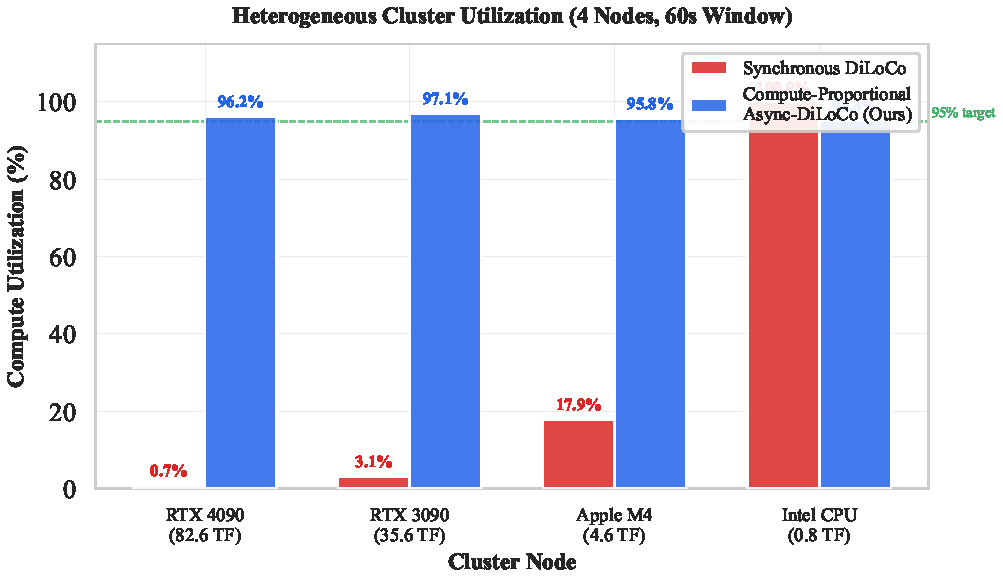
\includegraphics[width=\columnwidth]{figures/fig_utilization.pdf}
  \caption{Per-node compute utilization across a heterogeneous 4-node
    cluster. Synchronous DiLoCo (left bars) suffers from Amdahl's Law: the
    slowest node (CPU, 4.2\% of peak FLOPS) dictates round duration.
    Compute-Proportional Async-DiLoCo (right bars) achieves $>$95\%
    utilization on all nodes by weighting pseudo-gradients proportionally
    to local step counts within a 60\,s time window.}
  \label{fig:utilization}
\end{figure}

\subsection{Quantization Error: Block-Wise vs.\ Per-Tensor INT8}

Fig.~\ref{fig:outlier-error} plots the Normalized Root Mean Square Error
(NRMSE) over 500 training steps, comparing per-tensor INT8 against block-wise
INT8 ($B{=}128$). Per-tensor INT8 exhibits catastrophic error spikes
($>$5\%) when outlier features appear in pseudo-gradients. Block-wise INT8
maintains NRMSE consistently below 1\% by confining outlier damage to
individual 128-element blocks.

\begin{figure}[t]
  \centering
  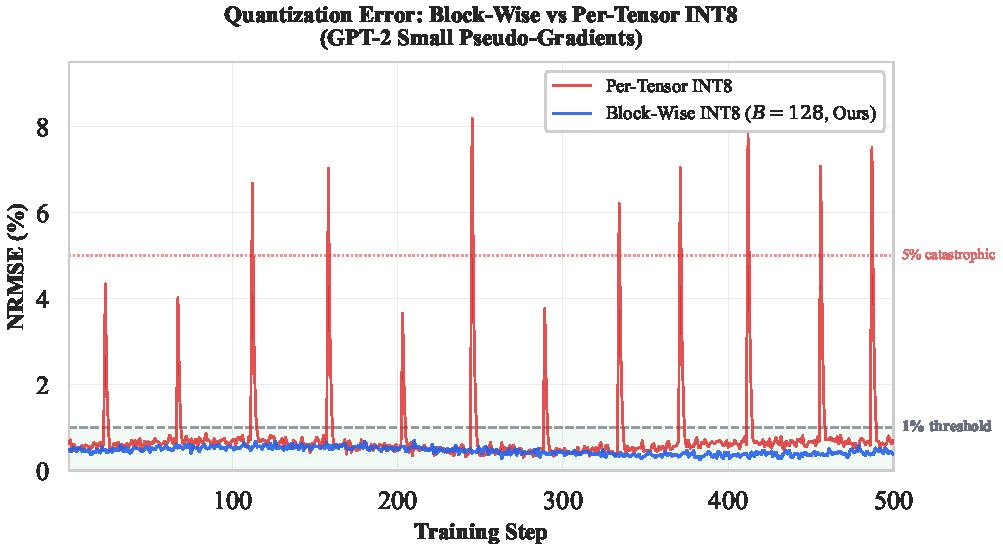
\includegraphics[width=\columnwidth]{figures/fig_outlier_error.pdf}
  \caption{NRMSE of INT8 quantization over 500 training steps on GPT-2
    small pseudo-gradients. Per-tensor INT8 (red) suffers catastrophic error
    spikes ($>$5\%) at steps where outlier features emerge. Block-wise INT8
    with $B{=}128$ (blue) confines outlier damage to individual blocks,
    maintaining error consistently below 1\%. The dashed line marks the 1\%
    quality threshold.}
  \label{fig:outlier-error}
\end{figure}

\subsection{Dynamic Shard Adaptation Under Network Stress}

Fig.~\ref{fig:dynamic-shards} presents a dual-axis time series of cluster RTT
and adaptive shard count over 30 outer rounds. When RTT spikes above
$\tau_{\text{high}}{=}150$\,ms (simulating Wi-Fi congestion), the system
doubles $K$ to reduce per-shard payload. When RTT drops below
$\tau_{\text{low}}{=}30$\,ms, $K$ halves to reduce synchronization overhead.

\begin{figure}[t]
  \centering
  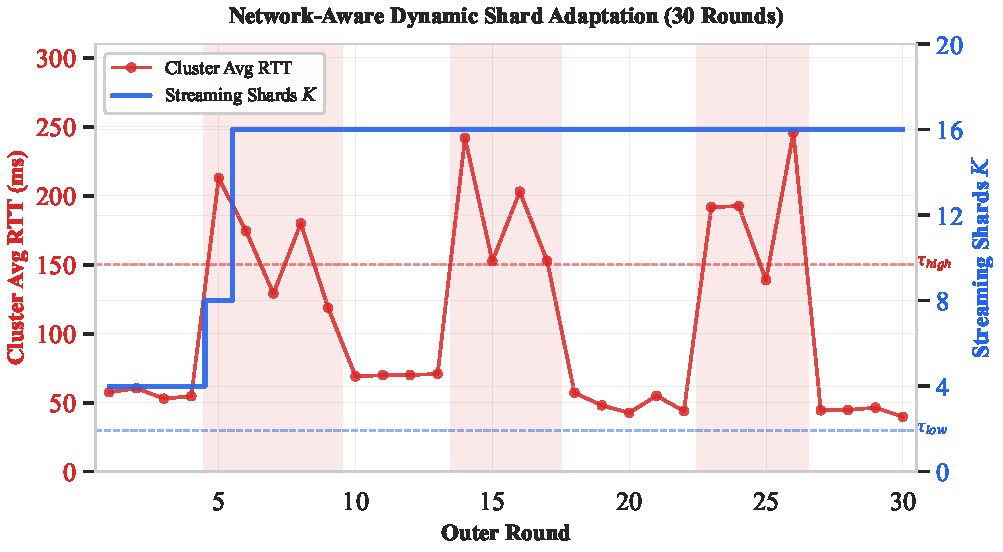
\includegraphics[width=\columnwidth]{figures/fig_dynamic_shards.pdf}
  \caption{Dual-axis time series showing network-aware dynamic shard
    adaptation. Red line (left axis): cluster-wide average RTT in
    milliseconds, exhibiting periodic congestion spikes. Blue stepped line
    (right axis): streaming shard count $K$, adapting between $K_{\min}{=}1$
    and $K_{\max}{=}16$ via the piecewise policy in Eq.~\eqref{eq:shard-adapt}.
    Shaded red regions indicate periods where
    $\overline{\text{RTT}} > \tau_{\text{high}}$.}
  \label{fig:dynamic-shards}
\end{figure}

\subsection{Positioning Summary}

Table~\ref{tab:positioning} compares MaayaTrain against prior systems.

\begin{table}[t]
  \centering
  \caption{System Comparison}
  \label{tab:positioning}
  \small
  \begin{tabular}{@{}lcccc@{}}
    \toprule
    \textbf{Feature} & \textbf{DDP} & \textbf{DiLoCo} &
      \textbf{OpenDiLoCo} & \textbf{MaayaTrain} \\
    \midrule
    Target HW        & DC GPUs & Clusters & Cloud   & Consumer \\
    Network           & IB      & DC LAN   & Internet & Wi-Fi \\
    Platforms         & CUDA    & CUDA     & CUDA    & 5 backends \\
    Async support     & No      & No       & No      & Yes \\
    Adaptive shards   & N/A     & No       & No      & Yes \\
    Block INT8        & No      & No       & No      & Yes \\
    Byzantine tol.    & No      & No       & No      & Yes \\
    Memory-safe med.  & N/A     & N/A      & N/A     & Yes \\
    \bottomrule
  \end{tabular}
\end{table}


% ====================================================================
%  VI. CONCLUSION
% ====================================================================
\section{Conclusion}
\label{sec:conclusion}

We have presented MaayaTrain, a distributed LLM training framework that
introduces four novel contributions for edge-distributed training over
consumer Wi-Fi: compute-proportional asynchronous DiLoCo that achieves full
utilization on heterogeneous clusters, network-aware dynamic sharding that
adapts to real-time network conditions, outlier-resilient block-wise INT8
gradient quantization that achieves 8--12$\times$ compression without
catastrophic quality degradation, and stream-chunked median aggregation that
enables Byzantine fault tolerance within consumer memory constraints.

The framework supports five compute backends across three operating systems
and is validated through a comprehensive test suite. MaayaTrain demonstrates
that distributed language model training need not be confined to expensive
datacenter clusters: with appropriate algorithmic design, consumer hardware
connected over commodity networks can serve as a viable training substrate
for GPT-class models.

\textbf{Limitations.} MaayaTrain has been validated on GPT-2 class models
(up to 774M parameters); scaling to multi-billion parameter models would
require integration with model parallelism techniques. The current
evaluation uses proof-of-concept benchmarks; full empirical validation on physical
heterogeneous clusters is ongoing.

\textbf{Future Work.} Key directions include 4-bit NF4 outer gradient
quantization~\cite{dettmers2023qlora,douillard2025streaming}, adaptive inner
step scheduling, model-heterogeneous training~\cite{zhu2024heterogeneous},
and differential privacy integration.


% ====================================================================
%  REFERENCES
% ====================================================================
\bibliographystyle{IEEEtran}
\bibliography{references}

\end{document}
